\section{La page d'accueil}

\begin{figure}[H]
\centering
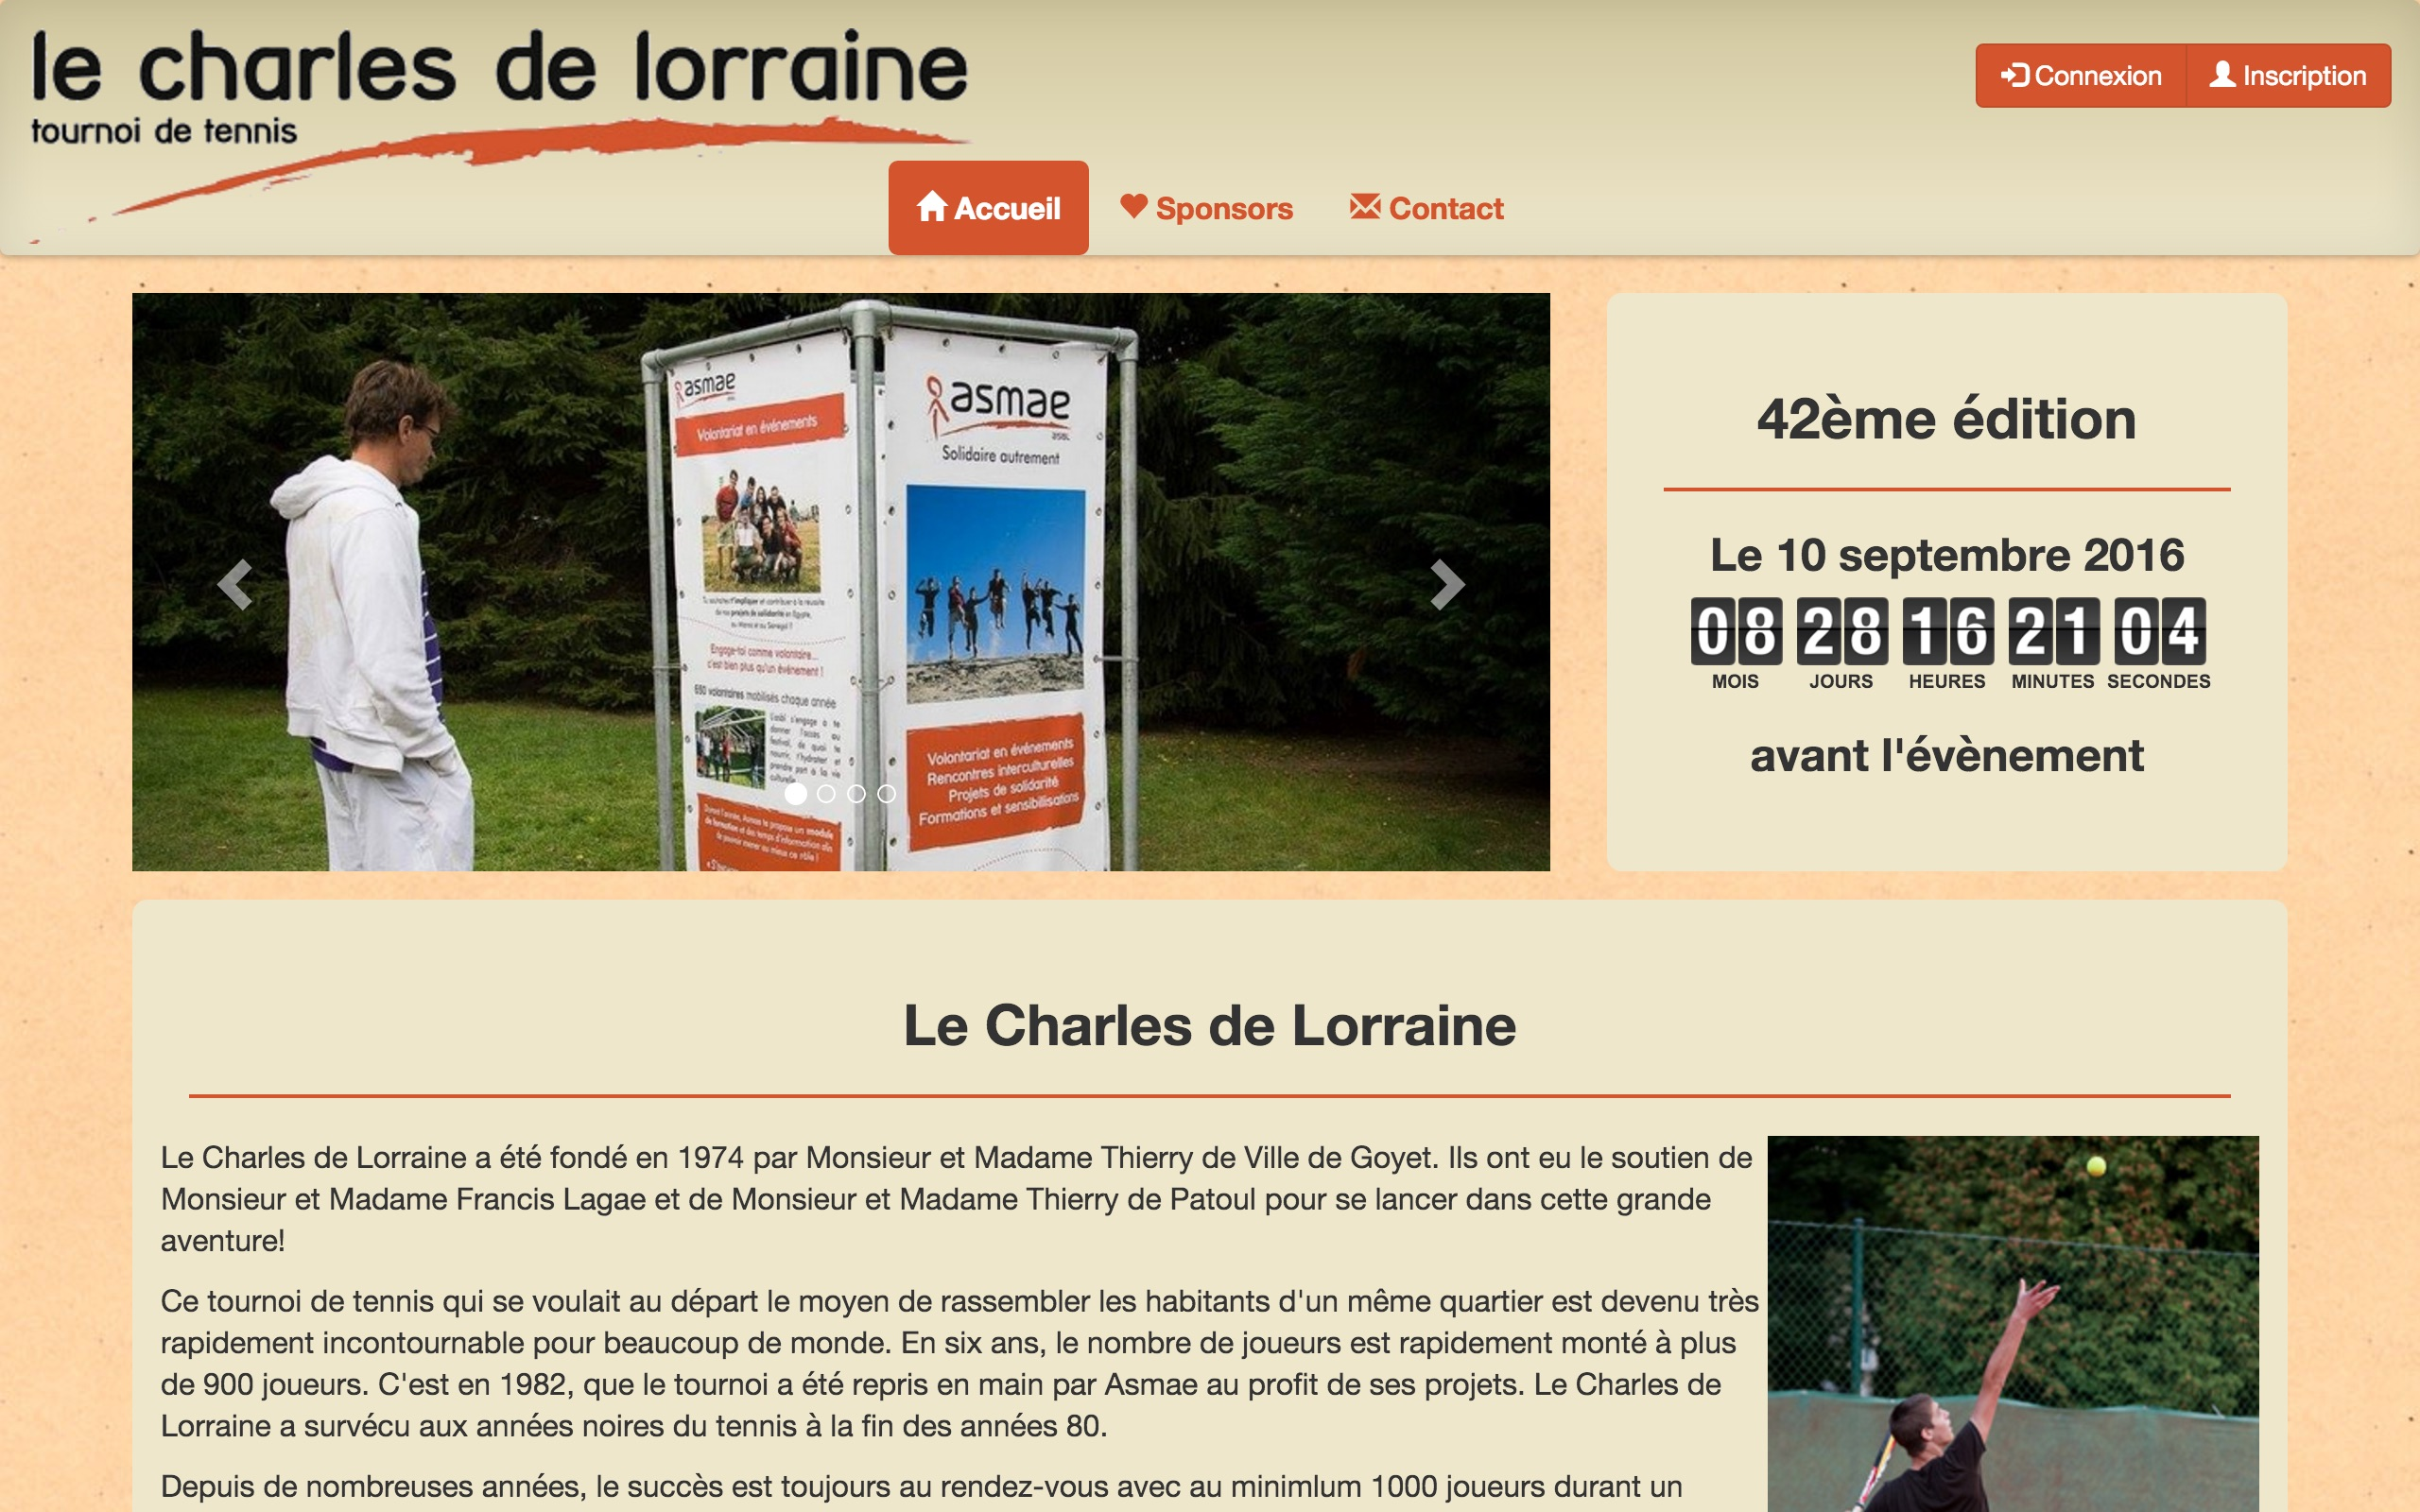
\includegraphics[scale=0.15]{page-accueil/page-accueil.jpg}
\caption{Page d'accueil}
\end{figure}

La page d'accueil est la première page accessible lorsque vous vous connectez au site web.\newline

Sur la page d'accueil, vous trouverez des photos des anciens tournois qui
défilent automatiquement. Vous pouvez également cliquer à droite ou à gauche
de ces images si vous souhaitez les revoir sans attendre un tour complet de
toutes les photos.\newline

Un décompte s'affiche sur votre écran. Il correspond à l'attente qu'il reste
jusqu'au début du prochain tournoi organisé par \textit{Le Charles de Lorraine}. Une
fois que le décompte sera terminé, vous pourrez accéder à une page qui
présentera les résultats du tournoi en cours.

\begin{figure}[H]
\centering

\includegraphics[scale=0.15]{page-accueil/page-accueil-decompte.jpg}
\caption{Page d'accueil - le décompte}
\end{figure}

Une description de l'évément se trouve au milieu de la page d'accueil. Elle permet d'en savoir plus sur l'histoire du tournoi, et vous
propose un lien pour avoir accès aux résultats des éditions précédentes, à la toute fin de la description.

\begin{figure}[H]
\centering
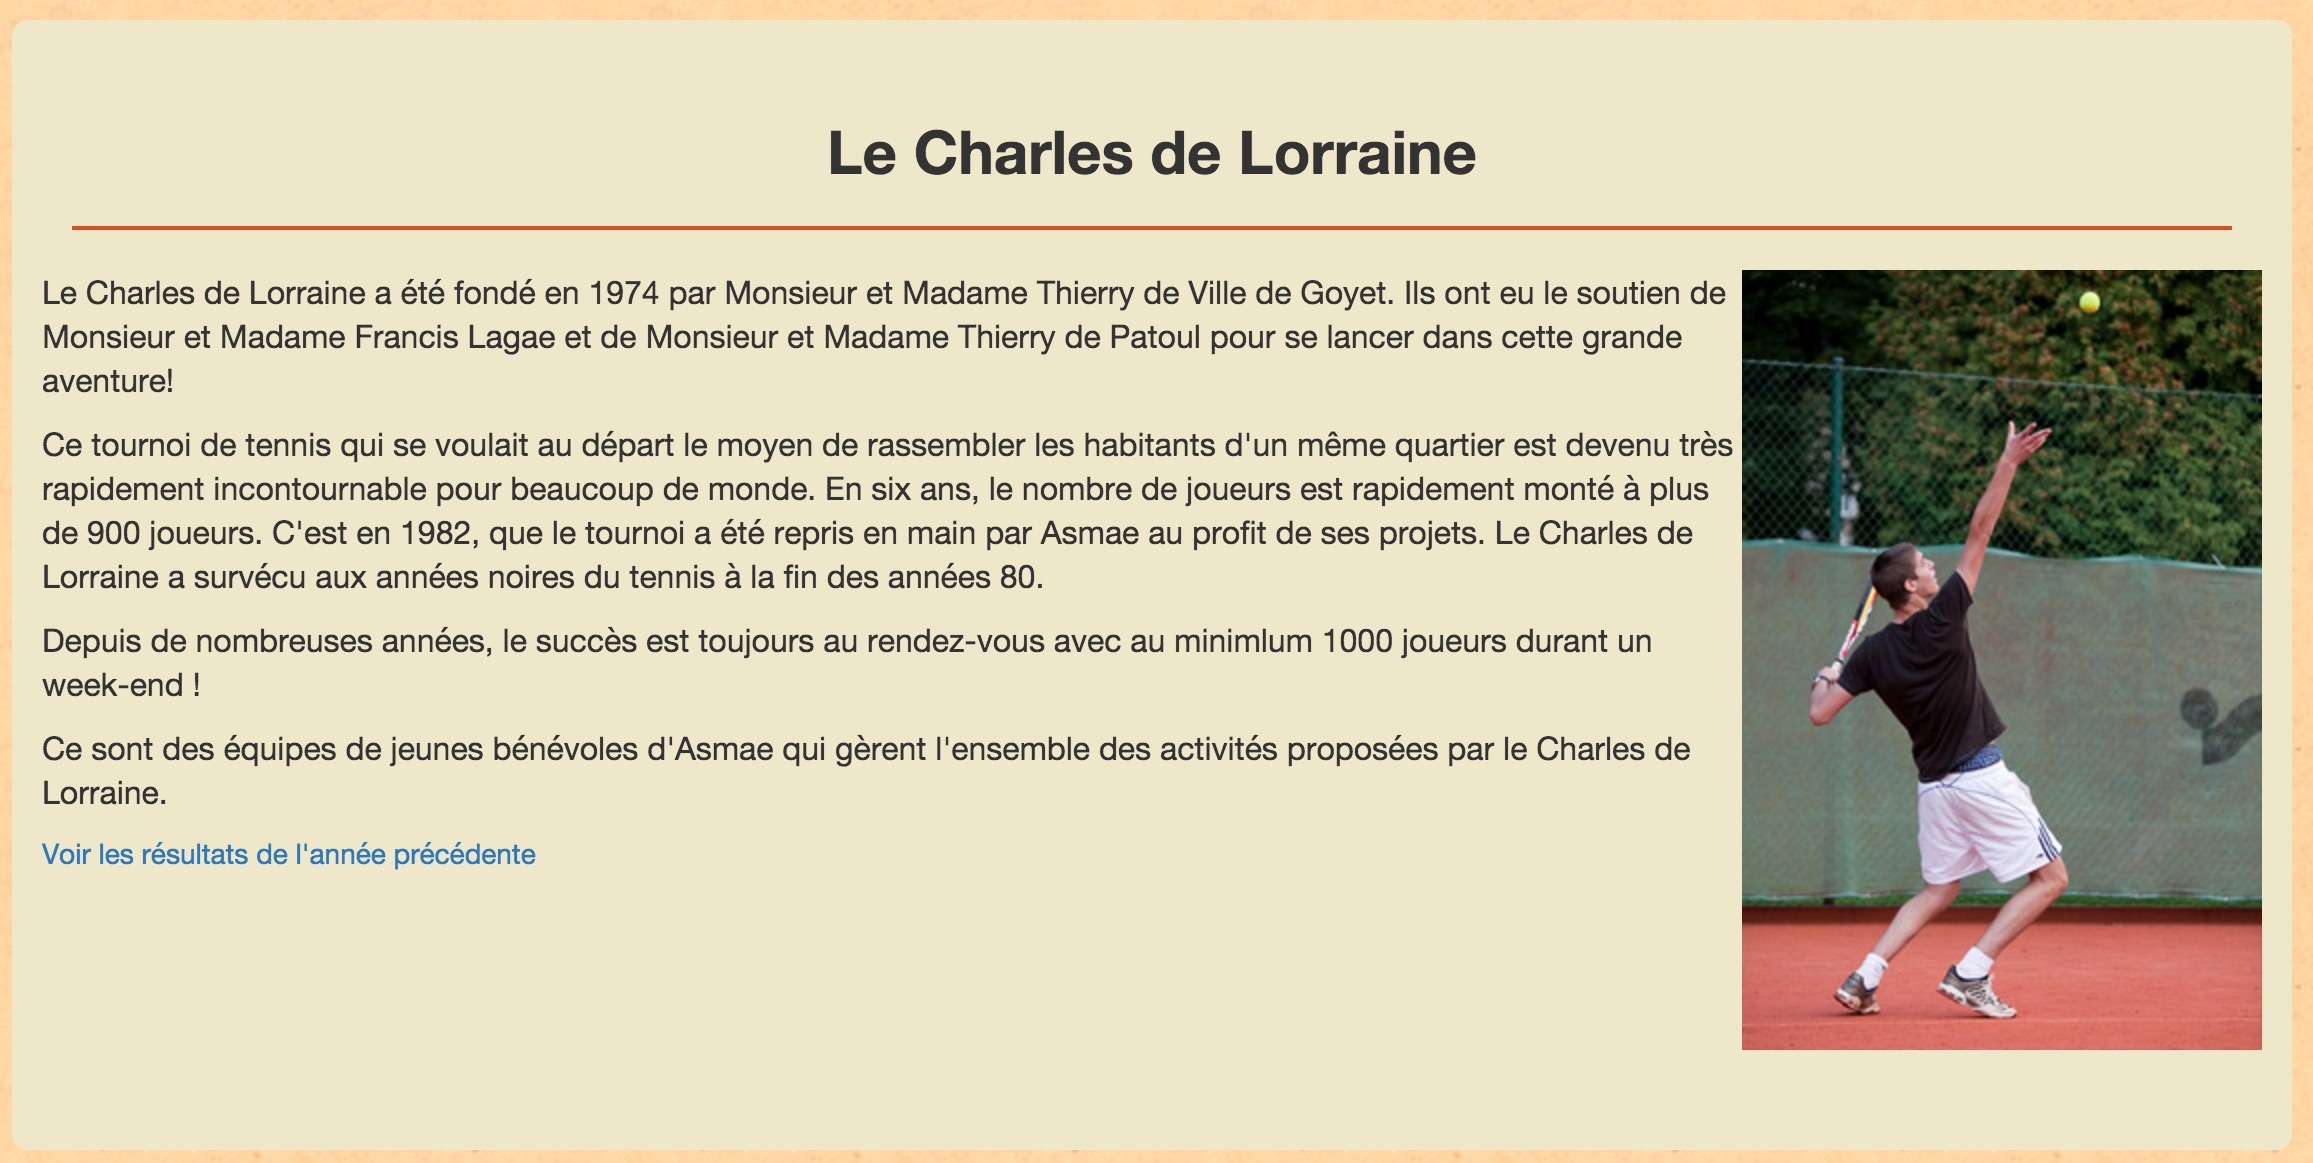
\includegraphics[scale=0.15]{page-accueil/page-accueil-description.jpg}
\caption{Page d'accueil - la description}
\end{figure}

Le \textit{Charles de Lorraine} souhaitent remercier les sponsors qui permettent
l'organisation du tournoi dans les meilleures conditions. Ceux-ci sont vitaux
pour l'association. Si vous souhaitez devenir un sponsor du \textit{Charles de Lorraine},
n'hésitez pas à nous envoyer un mail via notre formulaire de contact \ref{Page de contact}.

\begin{figure}[H]
\centering

\includegraphics[scale=0.15]{page-accueil/page-accueil-sponsors.jpg}
\caption{Page d'accueil - les sponsors}
\end{figure}

\subsection{Les résultats}

Les résultats sont classés par édition du tournoi, par jour de la semaine, et par catégorie du tournoi. Le nom du gagnant et des finalistes sont affichés pour chacun des tournois.

\begin{figure}[H]
\centering
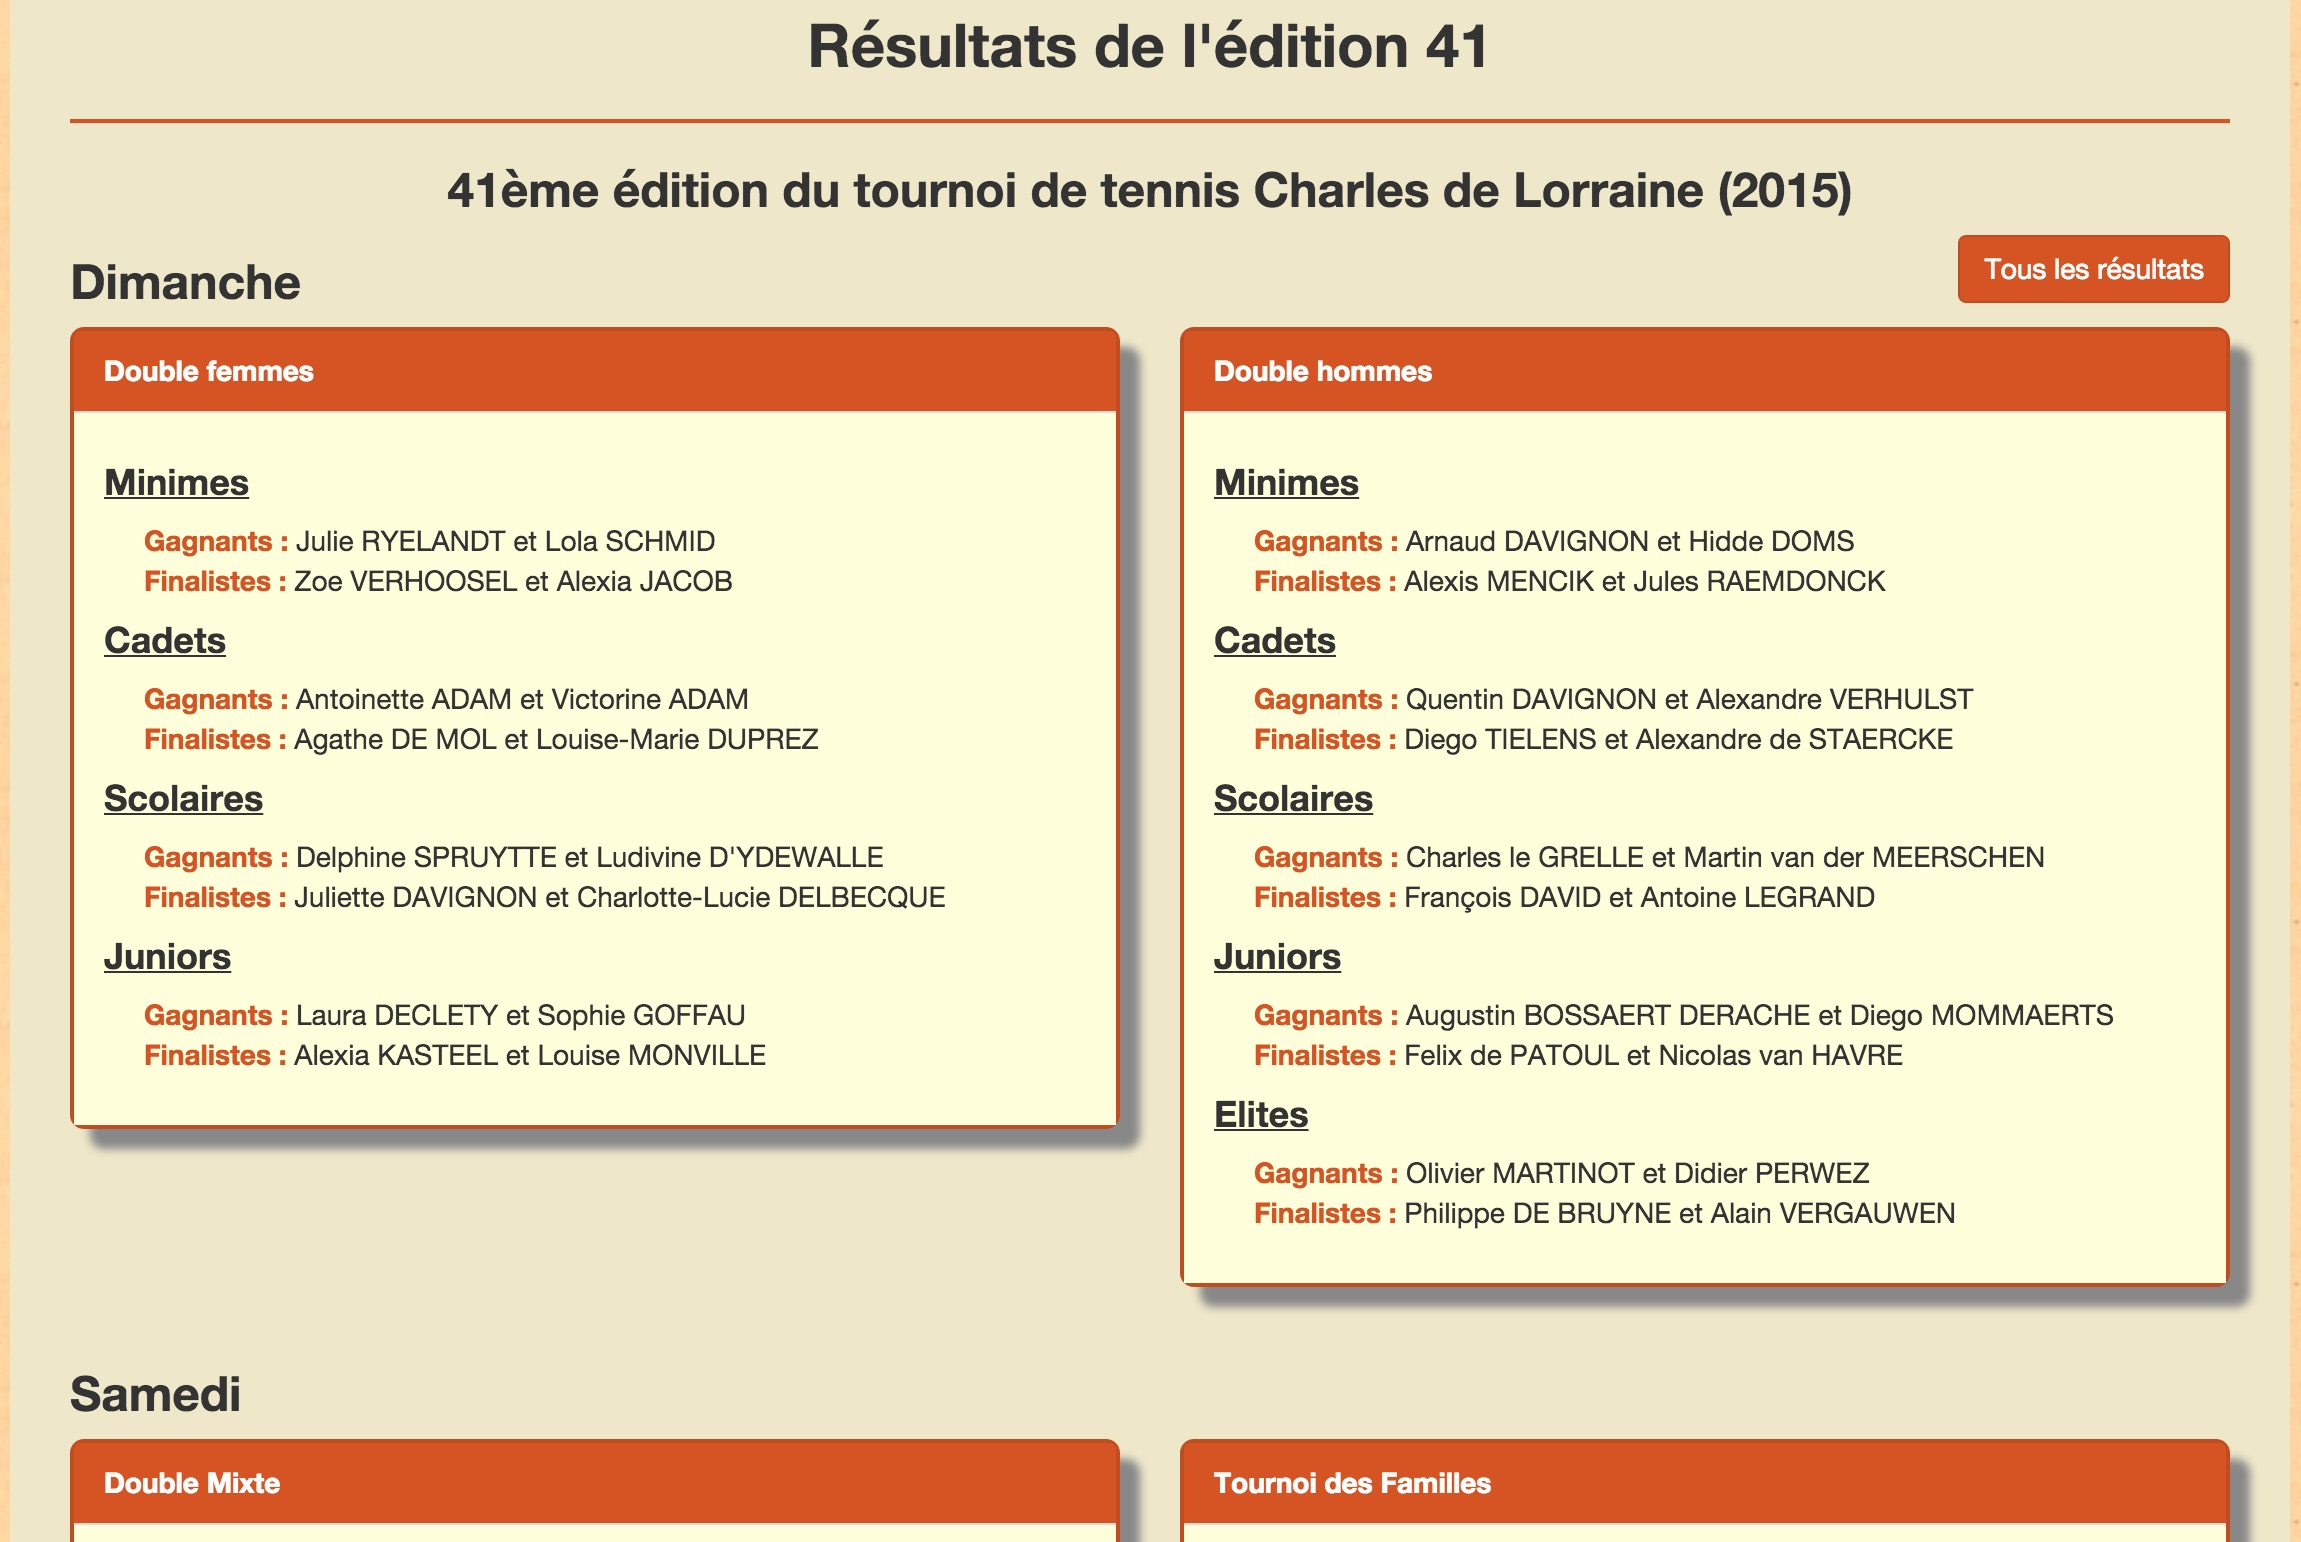
\includegraphics[scale=0.15]{page-accueil/page-accueil-resultats.jpg}
\caption{Page d'accueil - les résultats}
\end{figure}

